\chapterbegin{Interrupciones hardware}
\label{chp:Interrupciones}
\minitoc

{\bf Objetivos}: En esta sesión vamos a realizar programas que
utilizan dispositivos de E/S haciendo uso del sistema de
interrupciones hardware. Para poder programar los distintos parámetros
que configuran el entorno de las interrupciones es necesario conocer de
forma detallada cómo funcionan los registros asociados, ya que
éste es el mecanismo típico mediante el cual el procesador se
comunica con los periféricos.

Hacemos incapié en lo de {\it hardware} porque las
{\it interrupciones software} no son más que las llamadas a sistema
que vimos en el capítulo anterior. Ambas comparten vector de interrupciones,
pero las {\it interrupciones software} son más bien llamadas a subrutinas.

\section{Lectura previa}

El microprocesador se encuentra en un entorno donde existen otros
componentes. La forma de comunicación más usual entre estos
componentes y el microprocesador se denomina interrupción.
Básicamente, una interrupción es una petición que se hace a la CPU
para que detenga temporalmente el trabajo que esté realizando y
ejecute una rutina determinada. 

\subsection{El sistema de interrupciones del ARM}

Decimos que las interrupciones del ARM son {\bf autovectorizadas}.
Cada tipo de interrupción lleva asociado un número (que llamamos
{\bf número de interrupción}, $NI$) que identifica el tipo de servicio a
realizar. En total hay 8 tipos de interrupciones.
A partir de dicho número se calcula la dirección a la que salta la CPU
para atender dicha interrupción. A diferencia de otras arquitecturas
donde los vectores contienen las direcciones de las rutinas de
tratamiento, en ARM no tenemos datos sino instrucciones. Cada vector
contiene normalmente un salto a la rutina de tratamiento correspondiente.
Dicha rutina se suele llamar RTI ({\bf Rutina
de Tratamiento de Interrupción}). En la arquitectura ARMv6
todos los vectores de interrupción se almacenan en una zona de memoria
llamada {\bf tabla de vectores de interrupción}. Esta tabla comienza
en la dirección física 0x00000000 (aunque puede cambiarse por
0xffff0000) y acaba en 0x0000001f y contiene en total 8 vectores de
interrupción. Cuando termina de ejecutarse una RTI,
el procesador continúa ejecutando la instrucción siguiente a la que se
estaba ejecutando cuando se produjo la interrupción.

Existen dos tipos de interrupciones: hardware y software. Las {\bf
interrupciones hardware} son aquellas en las que su activación está
condicionada por el hardware del sistema, ya sea por: 1) {\it
excepciones} provocadas en la ejecución de alguna instrucción o error
grave, o 2) provocadas por la placa base o por cualquier tarjeta
implicada en un canal de E/S.

\noindent La lista del vector de interrupciones es la siguiente.

\begin{longtable}{ p{4.5cm} | p{2.5cm} | p{2cm} | p{4cm}}
\hline
{\bf Excepción} & {\bf Tipo} & {\bf Desplaz.} & {\bf Modo} \\ \hline
Reset                   & Interrupción & {\tt 0x00} & Supervisor \\ \hline
Instrucción no definida & Excepción & {\tt 0x04} & Indefinido \\ \hline
Interrupción software   & Int. software & {\tt 0x08} & Supervisor \\ \hline
Error en prefetch       & Excepción & {\tt 0x0C} & Abort \\ \hline
Error en datos          & Excepción & {\tt 0x10} & Abort \\ \hline
Reservado               & - & {\tt 0x14} & Reservado \\ \hline
IRQ                     & Interrupción & {\tt 0x18} & IRQ \\ \hline
FIQ                     & Interrupción & {\tt 0x1C} & FIQ \\ \hline
\caption{Vector de interrupciones}
\label{tab:excepciones}
\end{longtable}

La última columna se refiere al {\it Modo de operación} que comentamos en el primer
capítulo y que forma parte del registro {\tt cpsr} (ver figura \ref{fig:cpsr}).
Es un estado en el que se encuentra el procesador con una serie de privilegios
con respecto a otros modos y que gracias a ellos podemos construir un sistema operativo
con diferentes capas.

\begin{figure}[h]
  \centering
    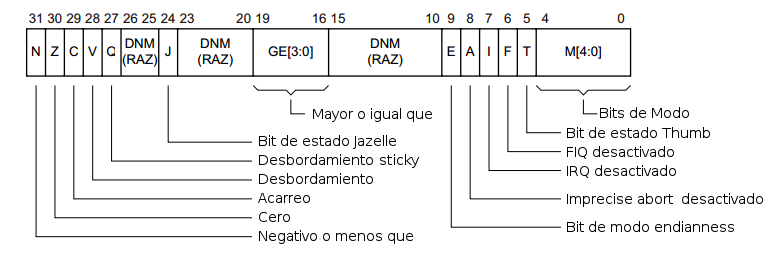
\includegraphics[width=14cm]{graphs/cpsr.png}
  \caption{Registro cpsr}
  \label{fig:cpsr}
\end{figure}

Cada modo tiene sus propios registros {\tt sp}, {\tt lr} y {\tt spsr}
(Saved Program Status Register) de tal
forma que no alteramos la pila ni los flags de la secuencia de programa que interrumpimos. Incluso
el modo {\tt FIQ} tiene 5 registros generales propios (desde {\tt r8} hasta {\tt r12}),
de esta forma si los empleamos en nuestra rutina de tratamiento no tendremos que
salvaguardarlos en pila. En la figura \ref{fig:tablareg} observamos los registros propios
mencionados marcados con un triángulo.

\begin{figure}[h]
  \centering
    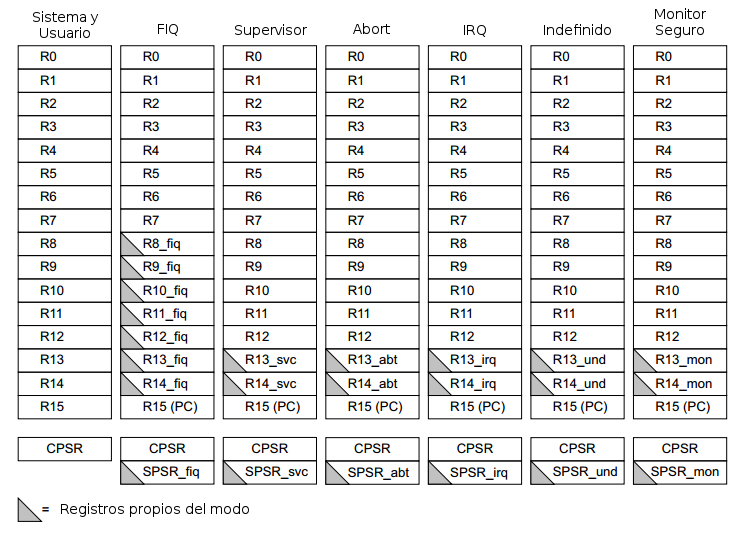
\includegraphics[width=14cm]{graphs/tablaregistros.png}
  \caption{Registros según modo de operación}
  \label{fig:tablareg}
\end{figure}

\begin{itemize}
  \item {\it Reset} es la excepción que permitiría un reset en caliente dentro de la CPU.
Desgraciadamente en la Raspberry no hay forma conocida de forzar esta excepción. Los pines
del conector {\tt P6} en la Raspberry 2.0 y {\tt RUN} en el modelo B+ (ver figura \ref{fig:pinReset})
provocan una secuencia completa de arranque, la que comienza con el bootloader de la GPU y acaba cediendo el control
a la CPU en la dirección 0x8000.

  \item {\it Instrucción no definida} se produce cuando en el flujo de instrucciones nos encontramos
un código de operación que no se corresponde con ninguna instrucción. Normalmente esto se
produce por una corrupción en la memoria de programa o bien que hemos saltado erróneamente
a una zona donde hay datos. También se puede dar el caso de que intentemos ejecutar código
ARM para una plataforma más moderna y nos encontremos con una instrucción no soportada por el
procesador que tenemos.

  \item Las {\it interrupciones software} son subrutinas que se incluyen en el
sistema operativo y que son llamadas desde el programa ejecutando la
instrucción {\tt swi \#n}. No interrumpen realmente nada, pero se
denominan así porque el mecanismo de funcionamiento es el mismo que en
las hardware.

  \item Luego tenemos los errores en {\it prefetch} y {\it datos}. Un error de {\it prefetch} se produce
cuando tratamos de ejecutar una instrucción que momentos antes hemos modificado. Es poco
frecuente y para que se produzca debemos escribir código que sea automodificable, que es
una práctica no deseable y apenas utilizada en dicha arquitectura. Los errores de {\it datos}
son generados normalmente por el manejador de memoria y responden a fallos de alineación, de
traslación, de dominio o de permisos.

  \item Lo siguiente es una entrada reservada, no tiene ninguna funcionalidad ahora
pero es probable que en futuras extensiones sí que la tenga.

  \item Por último están las excepciones que nos interesan y que trataremos en este capítulo, que son
las interrupciones normales {\tt IRQ} y las interrupciones rápidas {\tt FIQ}.
\end{itemize}

Puesto que cada interrupción, $NI$, lleva asociada una rutina, de
alguna forma, debe haber una correspondencia entre este $NI$
y la ubicación del vector asociado, que contiene la instrucción de salto a la rutina que debe
ejecutar cuando se produce la interrupción. La forma de hacerlo es multiplicar por
cuatro el número de interrupción para obtener un desplazamiento
($NI$*4). Se multiplica por 4 porque cada vector de excepción
ocupa 4 bytes (es lo que ocupa una instrucción en ARM).

Cuando se activa una interrupción, la CPU detiene su trabajo para
atenderla. Después, continúa su trabajo donde lo dejó. Los pasos a
seguir para que esto sea posible son:

\begin{enumerate}
  \item Cuando se activa la interrupción, se termina la ejecución de la
    instrucción en curso. A continuación hacemos una copia {\tt cpsr} en el registro
    propio {\tt spsr} correspondiente. De esta forma recordamos los flags de estado
    y el modo que había antes de la interrupción. Una vez hecha la copia se
    procede a cambiar {\tt cpsr}, conmutando al modo correspondiente
    según la tabla \ref{tab:excepciones}.

  \item Seguidamente a lo anterior almacenamos en {\tt lr} (en su registro propio del modo)
    el contenido de {\tt pc+8} (salvo si es un {\tt error en datos} que sería
    {\tt pc+12}). La razón de estos
    desplazamientos es puramente técnica, debido al segmentado de la CPU en
    el momento de hacer la copia el registro {\tt pc} se ha incrementado en 1 ó
    2 instrucciones.

\begin{longtable}{ p{1.8cm} | p{2cm} | p{5cm} }
\hline
{\bf PC} & {\bf Ins.} & {\bf Nombre} \\ \hline
x-4  & i-1 & Instrucción anterior \\ \hline
x & i & Instrucción interrumpida \\ \hline
x+4 & i+1 & Instrucción siguiente \\ \hline
x+8 & i+2 & ...     \\ \hline
x+12 & i+3 & ... \\ \hline
\end{longtable}

  \item Luego saltamos al vector correspondiente ($NI$*4). En esa posición del vector
    encontramos una instrucción de salto a la RTI correspondiente.

  \item Se ejecuta la rutina.

  \item La última instrucción de la rutina es {\tt subs pc, lr, \#4}, que se encarga
    de restaurar los flags originales y el modo copiando {\tt spsr} en {\tt cpsr}.
    Además volvemos al punto donde se interrumpió copiando de {\tt lr} a {\tt pc} (con el
    desplazamiento correspondiente).

   \item Se continúa ejecutando la tarea inicial.
\end{enumerate}

El registro {\tt cpsr} contiene 3 flags globales mediante los cuales podemos habilitar o
inhabilitar las interrupciones: uno para {\tt Abort} llamado {\tt A}, otro para
{\tt IRQ} llamado {\tt I} y el último para {\tt FIQ} denominado {\tt F}.

El manejo de estos flags corre a cuenta del usuario, en ningún momento la CPU enmascara
dichos flags. Por esta razón, si queremos dar prioridad a una interrupción en particular
para no ser interrumpidos nuevamente, debemos enmascarar dichos flags al comienzo de su RTI.

\subsection{Rutina de tratamiento de interrupción}

Es el segmento de código que se ejecuta para atender a una interrupción. Una vez se haya
ejecutado dicha rutina, retomamos la ejecución normal de nuestro programa, justo después de la instrucción
donde lo habíamos interrumpido. Cada rutina de tratamiento debe atender a todas las posibles
fuentes de interrupción de su mismo tipo, con lo que al comienzo de la interrupción se suelen
acceder a los registros asociados para detectar qué periférico ha causado la interrupción y
actuar en consecuencia.

Si nos interesan {\tt IRQ} y {\tt FIQ}, a lo sumo tendremos que escribir dos
rutinas de tratamiento distintas. Si se produce una {\tt IRQ}, se ejecutará el código
que se encuentre en la dirección {\tt 0x0018}, mientras que si lo que salta es una {\tt IRQ},
la dirección a ejecutar será {\tt 0x001C}. La diferencia entre una {\tt IRQ} y una
{\tt FIQ} es que esta última tiene sus propios registros desde {\tt r8} hasta {\tt r12}
asociados al modo de operación, con lo que podemos prescindir del salvado y recuperación
de estos registros en la RTI, ahorrando un tiempo que en determinadas aplicaciones de
tiempo real puede ser decisivo.

El esqueleto de una RTI es el siguiente.

\begin{lstlisting}
irq_handler:
        push    {lista registros}
        ...
        pop     {lista registros}
        subs    pc, lr, #4
\end{lstlisting}

Vemos que a diferencia de las subrutinas donde salíamos con {\tt lr}, en una RTI salimos
con {\tt lr-4} (si es un {\tt error en datos} sería {\tt lr-8}), a ello se debe que la última
instrucción sea {\tt subs} en lugar de {\tt movs}.
¿Y porqué hay un sufijo {\tt s} al final
de la instrucción {\tt sub}? Pues porque se trata de instrucción especial que sirve para
restaurar el registro {\tt cpsr} que había antes de la interrupción (copia {\tt spsr\_irq} o
{\tt spsr\_fiq} en {\tt cpsr}).

Imaginemos que el programa principal está en modo supervisor y que la interrupción que
esperamos el del tipo IRQ.
Cada modo de operación (en particular el modo IRQ) tiene 3 registros replicados: {\tt sp}, {\tt lr} y {\tt spsr}.
Para evitar confusiones los nombramos con los sufijos de modo {\tt \_svc} y {\tt \_irq} correspondientes.
Cuando ocurre una interrupción pasamos de modo supervisor a modo IRQ, pero antes hemos guardado
el registro {\tt cpsr} en {\tt spsr\_irq}.

Los registros {\tt sp\_svc} y {\tt lr\_svc} no se tocan para nada, con lo que no alteramos ni la
pila ni el registro de retorno del modo supervisor. El registro {\tt lr\_irq} se carga apuntando a la
instrucción {\tt i+2} siguiente a la que fue interrumpida, {\tt pc+8}. El resto de registros debemos salvarlos en pila si tenemos la intención
de modificarlos en nuestra RTI, al tener registro propio {\tt sp\_irq} se trata de una pila
independiente que no interfiere con la principal {\tt sp\_svc}. Luego se ejecuta el código
particular de la RTI, empleando a nuestro antojo los registros previamente salvados, y antes de
acabar la RTI recuperamos con su {\tt pop} correspondiente.

Al terminar la interrupción restauramos {\tt pc} partiendo {\tt lr\_irq} y {\tt cpsr} del registro
{\tt spsr\_irq}. Esto último fuerza un cambio de modo de IRQ a supervisor, conmutando {\tt sp} y {\tt lr}
a sus registros propios {\tt sp\_svc} y {\tt lr\_svc}. Con todo esto conseguimos volver exactamente
al punto del que partíamos minimizando las
operaciones que tiene que hacer la RTI y por tanto el retardo asociado. En otras arquitecturas
además de delegar en la RTI este trabajo, se usa la misma pila de programa, lo que puede
ocasionar problemas si nos importa lo que hay debajo de ésta.

\subsection{Pasos para configurar las interrupciones}

Nosotros vamos a tratar un caso sencillo de programa principal en el cual hacemos las
inicializaciones correspondientes para luego meternos en un bucle infinito y que las
interrupciones hagan su trabajo. Las cosas se pueden complicar metiendo código en
el programa principal concurrente con las interrupciones. Un ejemplo de esto sería
una rutina que dibuja la pantalla en el programa principal, mientras que se aceptan
interrupciones para registrar las pulsaciones del teclado.

Sin embargo nuestro programa principal tras la inicialización será una
instrucción que salta a sí misma continuamente, {\tt bucle: b bucle}.

El orden recomendado es el siguiente, aunque se puede cambiar el mismo salvo el último punto.

\begin{enumerate}
  \item Escribimos en el vector de interrupciones la instrucción de salto necesaria a nuestra RTI.
        Nosotros emplearemos una macro llamada {\tt ADDEXC} que tiene 2 parámetros, vector y
        dirección de la RTI. La macro genera y escribe el código de operación
        del salto, para ver los detalles consultar apéndice \ref{chp:MacroADDEXC}.
        En nuestros ejemplos tendremos IRQs ({\tt 0x18}) y FIQs ({\tt 0x1c}), por
        lo que como mucho haremos dos invocaciones a dicha macro (para dos RTIs distintas).
\begin{lstlisting}
      .macro    ADDEXC  vector, dirRTI
        ldr     r1, =(\dirRTI-\vector+0xa7fffffb)
        ror     r1, #2
        str     r1, [r0, #\vector]
      .endm
\end{lstlisting}
  \item Inicializamos el puntero de pila (registro {\tt sp}) en todos los modos de operación.
        Al cambiar el modo de operación hay que tener cuidado de no modificar la máscara
        global de interrupciones, ya que comparten el mismo byte bajo de {\tt cpsr}. Como
        sabemos que al comienzo estaban deshabilitadas, las mantenemos igual (bits {\tt I}
        y {\tt F} a 1.
        Los punteros tienen que alojar la pila en zonas distintas donde sepamos que no
        habrá conflictos con la memoria de programa. En los ejemplos en los que usemos FIQ e
        IRQ inicializamos la pila de FIQ
        a {\tt 0x4000}, la de IRQ a {\tt 0x8000} y la del modo Supervisor a {\tt 0x8000000}.
        Como la memoria de programa empieza en {\tt 0x8000} y la pila crece hacia abajo,
        tendremos 16K de pila en modo IRQ, otros 16K en modo FIQ y 128Mb a compartir entre
        programa principal y pila de programa. El mapa de memoria sería el indicado en la figura
        \ref{fig:mapamemoria}

\begin{figure}[h]
  \centering
    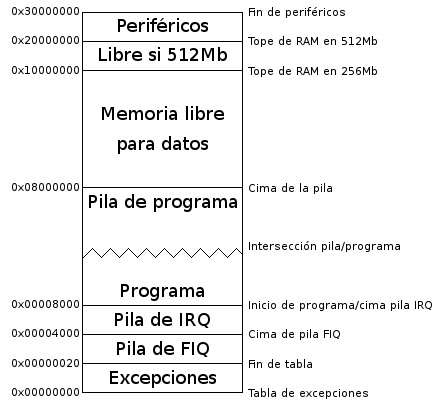
\includegraphics[width=14cm]{graphs/mapamemoria.png}
  \caption{Mapa de memoria en nuestros ejemplos}
  \label{fig:mapamemoria}
\end{figure}

  \item Escribimos código de inicialización ajeno al proceso de interrupción, como por ejemplo
        configurar los GPIOs a salidas donde queramos que actúe un LED.
  \item Ahora viene la inicialización de las interrupciones. Aquí le decimos al sistema qué fuentes
        pueden provocar interrupciones, escribiendo en los registros asociados. 
  \item El último paso es habilitar las interrupciones globalmente escribiendo en el registro
        {\tt cpsr}. Lo hacemos indirectamente vía otro registro, y la instrucción tiene otro
        nombre pero hace lo mismo que un {\tt mov}. En concreto se llama {\tt msr}, y también hay
        otra equivalente {\tt mrs} si lo que queremos es leer de {\tt cpsr} a un registro.
  \item Después de esto se acaba la inicialización y tendríamos el bucle infinito del que consta
        nuestro programa principal. Si todo ha ido bien las rutinas de tratamiento de interrupción
        se encargarán de hacer funcionar nuestro programa como queramos.
\end{enumerate}

\subsection{El controlador de interrupciones}

Los registros que componen el controlador de interrupciones son los siguientes.

\begin{figure}[h]
  \centering
    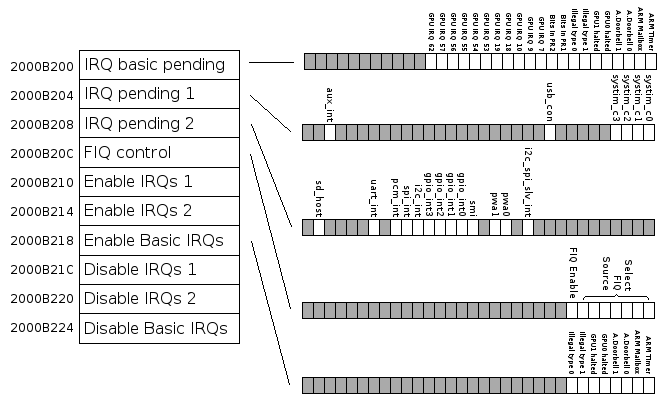
\includegraphics[width=14cm]{graphs/interrupciones.png}
  \caption{Interrupciones}
  \label{fig:interrupciones}
\end{figure}

Las {\tt FIQs} sólo tienen un registro de control asociado, quedando todo el detalle
en las {\tt IRQs}. Hay tres grupos de tres
registros cada uno. El primer grupo (Pending) sirve para indicar que hay una interrupción
pendiente, el segundo (Enable) es para habilitar las interrupciones y el tercero (Disable)
para deshabilitarlas. Dentro de cada grupo tenemos un registro básico que tiene un resumen
sobre el mapa de interrupciones y otros dos registros que
indican con más detalle la fuente de la interrupción. En el registro básico
hay fuentes individuales {\tt GPU IRQ x} y bits que engloban a varias fuentes {\tt Bits in PR1},
que por ejemplo indica que el origen hay que buscarlo en el registro 1. En el registro 1 están
las primeras 32 posiciones del mapa de interrupciones, mientras que en el registro 2 están
las 32 últimas.

La documentación oficial sobre el mapa de interrupciones está incompleta, pero buscando un poco
por internet se puede encontrar que las interrupciones asociadas al {\tt System Timer} se
controlan con los 4 primeros bits de la tabla (uno para cada comparador).

En la figura \ref{fig:interrupcionesgrupos} vemos los registros ordenados en grupos.

\begin{figure}[h]
  \centering
    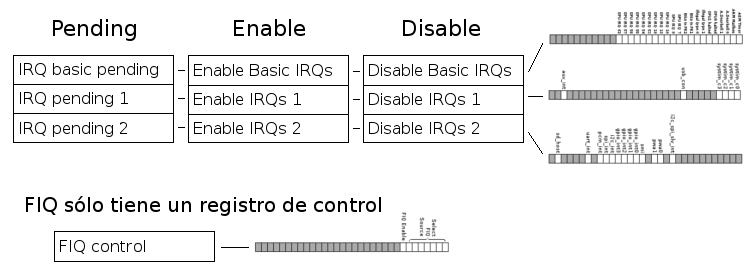
\includegraphics[width=15cm]{graphs/interrupcionesgrupos.png}
  \caption{Agrupación de registros de interrupciones}
  \label{fig:interrupcionesgrupos}
\end{figure}

La forma habitual de trabajar es usar el registro apropiado del grupo {\tt Enable} para
habilitar la fuente de interrupción que queramos que nos interrumpa. Luego en el caso de
ser interrumpidos podemos detectar cuál ha sido la fuente leyendo el mismo bit del
grupo {\tt Pending} y finalmente, si pasamos a otra sección del programa donde no queremos
que nos interrumpa más dicha fuente la desactivamos con el grupo {\tt Disable}.

A parte del controlador de interrupciones, cada dispositivo tiene su propio mecanismo de
habilitar/deshabilitar y detectar/notificar la fuente de interrupción. En el caso del GPIO tenemos
los registros {\tt GPRENn}, {\tt GPFENn}, {\tt GPHENn}, {\tt GPLENn}, {\tt GPARENn} y {\tt GPAFENn}
para habilitar/deshabilitar. Para detectar/notificar están los {\tt GPEDSn}.

Para el temporizador tenemos que {\tt STCS} hace las funciones de detección y notificación. No
existen registros específicos para habilitar/deshabilitar ya que el controlador de
interrupciones permite habilita/deshabilitar cada comparador por separado.

El único registro que nos falta por ver es {\tt FIQ control ó INTFIQCON} que hemos
mostrado en la figura \ref{fig:interrupciones}. Antes mostraremos la lista de fuentes
de interrupción aplicables a este registro.

\begin{longtable}{ p{2cm} | p{6cm}}
\hline
{\bf Índice} & {\bf Fuente} \\ \hline
0-63  & Interrupciones IRQ 1 y 2 (ver figura \ref{fig:interrupciones})  \\ \hline
64    & ARM Timer  \\ \hline
65    & ARM Mailbox \\ \hline
66    & ARM Doorbell 0 \\ \hline
67    & ARM Doorbell 1 \\ \hline
68    & GPU0 detenida \\ \hline
69    & GPU1 detenida \\ \hline
70    & Acceso ilegal de tipo 1 \\ \hline
71    & Acceso ilegal de tipo 2 \\ \hline
\end{longtable}

Son las mismas fuentes que en IRQ pero condensadas en un único registro. De 0 a 31 coincide
con la tabla {\tt IRQ 1}, de 32 a 63 con {\tt IRQ 2} y de 64 en adelante con {\tt IRQ Basic}.

El registro {\tt INTFIQCON} se programa con los 8 bits inferiores, indicando en el bit 7 si
queremos habilitar la fuente, y en los bits del 0 al 6 ponemos el índice de la fuente que
se corresponde con la lista. A diferencia de las IRQ, con las FIQ sólo podemos atender a
una fuente de interrupción. 

\subsection{Ejemplo. Encender LED rojo a los 4 segundos}

Se trata de programar el comparador y las interrupciones para que
transcurrido un tiempo determinado se produzca una interrupción, dentro
de la cual se encienda el LED. Es un caso muy sencillo porque sólo
se va a producir una interrupción que viene de una sola fuente, por
lo que en la RTI lo único que haremos es encender el LED.

El diagrama que vamos a usar es el siguiente.

\begin{figure}[h]
  \centering
    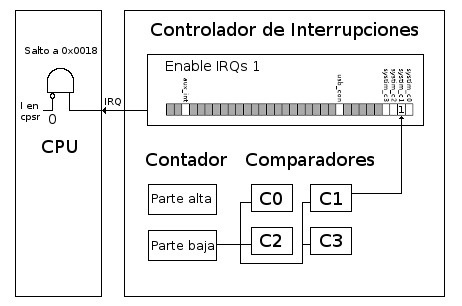
\includegraphics[width=14cm]{graphs/inter1.png}
  \caption{Interrupciones}
  \label{fig:inter1}
\end{figure}

\subsubsection{1. Escribimos en el vector de interrupciones}

  Invocamos la macro para una IRQ, pasándole la etiqueta de nuestra RTI {\tt irq\_handler}.
\begin{lstlisting}
        ADDEXC  0x18, irq_handler
\end{lstlisting}

\subsubsection{2. Inicializamos punteros de pila}

La única forma de acceder a los registros {\tt sp\_irq} y {\tt sp\_fiq} es cambiando de modo
 y modificando el registro {\tt sp} correspondiente.

El modo viene indicado en la parte más baja del registro {\tt cpsr}, el cual modificaremos
con la instrucción especial {\tt msr}. En la figura \ref{fig:cpsr} vemos el contenido completo
del registro {\tt cpsr}. Como {\tt cpsr} es un registro muy heterogéneo, usamos
sufijos para acceder a partes concretas de él. En nuestro caso sólo nos
interesa cambiar el byte bajo del registro, añadimos el sufijo {\tt \_c} llamándolo {\tt cpsr\_c},
para no alterar el resto del registro. Esta parte comprende el modo de operación
y las máscaras globales de las interrupciones. Otra referencia útil es {\tt cpsr\_f} que modifica
únicamente la parte de flags (byte alto). Las otras 3 referencias restantes apenas se usan y
son {\tt cpsr\_s} (Status) para el tercer byte, {\tt cpsr\_x} (eXtended) para el segundo byte y
{\tt cpsr\_csxf} para modificar los 4 bytes a la vez.

En la siguiente tabla vemos cómo se codifica el modo de operación.

\begin{longtable}{ p{1.8cm} | p{2cm} | p{5cm} | p{1cm} | p{1cm} }
\hline
{\bf Hex} & {\bf Binario} & {\bf Modo de operación} \\ \hline
0x10 & 10000 & Usuario        \\ \hline
0x11 & 10001 & FIQ            \\ \hline
0x12 & 10010 & IRQ            \\ \hline
0x13 & 10011 & Supervisor     \\ \hline
0x16 & 10110 & Monitor seguro \\ \hline
0x17 & 10111 & Abort          \\ \hline
0x1B & 11011 & Indefinido     \\ \hline
0x1F & 11111 & Sistema        \\ \hline
\end{longtable}

Como las interrupciones globales de IRQ y FIQ están desactivadas (estado por defecto tras
el reset), mantenemos a 1 dichos bits.

El código que inicializa los punteros de pila es el siguiente.

\begin{lstlisting}
        mov     r0, #0b11010010   @modo IRQ, FIQ&IRQ desact
        msr     cpsr_c, r0
        mov     sp, #0x8000
        mov     r0, #0b11010011   @modo SVC, FIQ&IRQ desact
        msr     cpsr_c, r0
        mov     sp, #0x8000000
\end{lstlisting}

En concreto a {\tt 0x8000} y {\tt 0x8000000} para los modos {\tt IRQ} y
{\tt Supervisor} respectivamente.

\subsubsection{3. Código de inicialización ajeno a interrupciones}

En el ejemplo que tenemos entre manos se trata de configurar los puertos
GPIO de entrada y de salida, inicializar temporizadores. En casos más complejos tendríamos que
inicializar estructuras de datos, rellenar las tablas que sean precalculadas y en general
cualquier tarea de inicialización requerida para hacer funcionar nuestro programa.

El código para asignar el sentido al pin GPIO 9 es el siguiente.

\begin{lstlisting}
        ldr     r0, =GPBASE
/* guia bits           xx999888777666555444333222111000*/
        mov     r1, #0b00001000000000000000000000000000
        str     r1, [r0, #GPFSEL0]
\end{lstlisting}

Luego programamos el comparador para que salte la interrupción a los 4,19 segundos.

\begin{lstlisting}
        ldr     r0, =STBASE
        ldr     r1, [r0, #STCLO]
        add     r1, #0x400000     @4,19 segundos
        str     r1, [r0, #STC1]
\end{lstlisting}

\subsubsection{4. Inicializamos interrupciones localmente}

Consiste en escribir en los registros asociados dependiendo de las fuentes que querramos
activar. En este primer ejemplo habilitamos el comparador
{\tt C1} del temporizador como fuente de interrupción.

\begin{lstlisting}
        ldr     r0, =INTBASE
        mov     r1, #0b0010
        str     r1, [r0, #INTENIRQ1]
\end{lstlisting}

\subsubsection{5. Habilitamos interrupciones globalmente}

Se trata de poner a cero el bit correspondiente en {\tt cpsr}. El siguiente código habilita
interrupciones del tipo IRQ.

\begin{lstlisting}
        mov     r0, #0b01010011   @modo SVC, IRQ activo
        msr     cpsr_c, r0
\end{lstlisting}

\subsubsection{6. Resto del programa principal}

Como hemos adelantado, en todos nuestros ejemplos será un bucle infinito.

\begin{lstlisting}
bucle:  b       bucle
\end{lstlisting}

A continuación mostramos el listado del ejemplo completo.

\begin{lstlisting}[caption={inter1.s},label={lst:codigoPract5_1}]
        .include  "inter.inc"
.text
        ADDEXC  0x18, irq_handler
        mov     r0, #0b11010010   @modo IRQ, FIQ&IRQ desact
        msr     cpsr_c, r0
        mov     sp, #0x8000
        mov     r0, #0b11010011   @modo SVC, FIQ&IRQ desact
        msr     cpsr_c, r0
        mov     sp, #0x8000000
        ldr     r0, =GPBASE
/* guia bits           xx999888777666555444333222111000*/
        mov     r1, #0b00001000000000000000000000000000
        str     r1, [r0, #GPFSEL0]
        ldr     r0, =STBASE
        ldr     r1, [r0, #STCLO]
        add     r1, #0x400000     @4,19 segundos
        str     r1, [r0, #STC1]
        ldr     r0, =INTBASE
        mov     r1, #0b0010
        str     r1, [r0, #INTENIRQ1]
        mov     r0, #0b01010011   @modo SVC, IRQ activo
        msr     cpsr_c, r0
bucle:  b       bucle

irq_handler:
        push    {r0, r1}
        ldr     r0, =GPBASE
/* guia bits           10987654321098765432109876543210*/
        mov     r1, #0b00000000000000000000001000000000
        str     r1, [r0, #GPSET0]
        pop     {r0, r1}
        subs    pc, lr, #4
\end{lstlisting}

Observamos que la RTI es muy sencilla, aparte del esqueleto tenemos tres instrucciones
encargadas de encender el LED en cuestión.

\subsection{Ejemplos de aplicación}

Vamos a crear un archivo {\tt inter.inc} donde guardaremos las constantes
asociadas a los registros y también la macro {\tt ADDEXC}, esta última
se explica en detalle en el apéndice \ref{chp:MacroADDEXC}. De esta forma evitamos escribir
siempre las mismas constantes, haciendo el código más sencillo de mantener.

\begin{lstlisting}[caption={inter.inc},label={lst:codigoPract5_0}]
      .macro    ADDEXC  vector, dirRTI
        ldr     r1, =(\dirRTI-\vector+0xa7fffffb)
        ror     r1, #2
        str     r1, [r0, #\vector]
      .endm
        .set    GPBASE,   0x20200000
        .set    GPFSEL0,        0x00
        .set    GPFSEL1,        0x04
        .set    GPFSEL2,        0x08
        .set    GPSET0,         0x1c
        .set    GPCLR0,         0x28
        .set    GPEDS0,         0x40
        .set    GPREN0,         0x58
        .set    GPPUD,          0x94
        .set    GPPUDCLK0,      0x98
        .set    STBASE,   0x20003000
        .set    STCS,           0x00
        .set    STCLO,          0x04
        .set    STC1,           0x10
        .set    STC3,           0x18
        .set    INTBASE,  0x2000b000
        .set    INTFIQCON,     0x20c
        .set    INTENIRQ1,     0x210
        .set    INTENIRQ2,     0x214
\end{lstlisting}

El método para incluir el código fuente de un fichero dentro de otro es mediante
la macro {\tt .include}, todos nuestros ficheros comienzarán con lo siguiente.

\begin{lstlisting}
        .include  "inter.inc"
\end{lstlisting}

\subsection{Parpadeo de todos los LEDs}

Sería hacer lo mismo que en la lección anterior pero empleando interrupciones y aplicando
la salida simultáneamente a los 6 LEDs en lugar de sólo al primero. La novedad en lo
que a interrupciones se refiere consiste en reprogramar el comparador C1 cada vez que
se produzca una interrupción, de esta forma conseguimos interrupciones periódicas en lugar
de una única interrupción.

Veamos el código.

\begin{lstlisting}[caption={inter2.s},label={lst:codigoPract5_2}]
        .include  "inter.inc"
.text
        ADDEXC  0x18, irq_handler
        mov     r0, #0b11010010   @modo IRQ, FIQ&IRQ desact
        msr     cpsr_c, r0
        mov     sp, #0x8000
        mov     r0, #0b11010011   @modo SVC, FIQ&IRQ desact
        msr     cpsr_c, r0
        mov     sp, #0x8000000
        ldr     r0, =GPBASE
        mov     r1, #0b00001000000000000000000000000000
        str     r1, [r0, #GPFSEL0]
/* guia bits           xx999888777666555444333222111000*/
        ldr     r1, =0b00000000001000000000000000001001
        str     r1, [r0, #GPFSEL1]
        ldr     r1, =0b00000000001000000000000001000000
        str     r1, [r0, #GPFSEL2]
        ldr     r0, =STBASE
        ldr     r1, [r0, #STCLO]
        add     r1, #2
        str     r1, [r0, #STC1]
        ldr     r0, =INTBASE
        mov     r1, #0b0010
        str     r1, [r0, #INTENIRQ1]
        mov     r0, #0b01010011   @modo SVC, IRQ activo
        msr     cpsr_c, r0
bucle:  b       bucle

irq_handler:
        push    {r0, r1, r2}
        ldr     r0, =ledst
        ldr     r1, [r0]
        eors    r1, #1
        str     r1, [r0]
        ldr     r0, =GPBASE
/* guia bits           10987654321098765432109876543210*/
        ldr     r1, =0b00001000010000100000111000000000
        streq   r1, [r0, #GPSET0]
        strne   r1, [r0, #GPCLR0]
        ldr     r0, =STBASE
        mov     r1, #0b0010
        str     r1, [r0, #STCS]
        ldr     r1, [r0, #STCLO]
        ldr     r2, =500000       @1 Hz
        add     r1, r2
        str     r1, [r0, #STC1]
        pop     {r0, r1, r2}
        subs    pc, lr, #4

ledst:  .word   0
\end{lstlisting}

Y vamos enumerando, por orden, los pasos que hemos seguido. En primer lugar apuntamos a nuestra
RTI en el vector de interrupciones.

\begin{lstlisting}
        ADDEXC  0x18, irq_handler
\end{lstlisting}

Luego inicializamos los punteros de pila.

\begin{lstlisting}
        mov     r0, #0b11010010   @modo IRQ, FIQ&IRQ desact
        msr     cpsr_c, r0
        mov     sp, #0x8000
        mov     r0, #0b11010011   @modo SVC, FIQ&IRQ desact
        msr     cpsr_c, r0
        mov     sp, #0x8000000
\end{lstlisting}

Lo siguiente es configurar los pines GPIO asociados a los 6 LEDs como salidas.

\begin{lstlisting}
        ldr     r0, =GPBASE
        mov     r1, #0b00001000000000000000000000000000
        str     r1, [r0, #GPFSEL0]
/* guia bits           xx999888777666555444333222111000*/
        ldr     r1, =0b00000000001000000000000000001001
        str     r1, [r0, #GPFSEL1]
        ldr     r1, =0b00000000001000000000000001000000
        str     r1, [r0, #GPFSEL2]
\end{lstlisting}

Preparamos el comparador {\tt C1} para que al cabo de dos microsegundos nos proporcione la primera
interrupción.

\begin{lstlisting}
        ldr     r0, =STBASE
        ldr     r1, [r0, #STCLO]
        add     r1, #2
        str     r1, [r0, #STC1]
\end{lstlisting}

Para después habilitar las interrupciones asociadas al comparador {\tt C1}.

\begin{lstlisting}
        ldr     r0, =INTBASE
        mov     r1, #0b0010
        str     r1, [r0, #INTENIRQ1]
\end{lstlisting}

Y finalmente habilitar las interrupciones {\tt IRQ} globalmente, entrando luego en
el bucle infinito.

\begin{lstlisting}
        mov     r0, #0b01010011   @modo SVC, IRQ activo
        msr     cpsr_c, r0
bucle:  b       bucle
\end{lstlisting}

Ya hemos terminado con el programa principal, que como veremos más adelante va a ser
siempre muy parecido.

Lo interesante está en la RTI, que es donde hacemos parpadear los LEDs y configuramos
el comparador para la siguiente interrupción.

El estado de los LEDs (si están apagados o encendidos) lo guardamos en la variable
{\tt ledst}, que conmutamos entre cero y uno mediante un {\tt OR} exclusivo. Al
actualizar los {\tt flags} tras esta operación, tenemos que si el resultado fue
cero nos lo indica el {\tt flag Z} activo, mientras que estará inactivo en el
caso contrario (resultado 1). Mediante las instrucciones de ejecución condicional
{\tt streq} y {\tt strne} enviamos la orden al puerto que enciende los LEDs o al
puerto que los apaga, respectivamente.

\begin{lstlisting}
irq_handler:
        push    {r0, r1, r2}
        ldr     r0, =ledst
        ldr     r1, [r0]
        eors    r1, #1
        str     r1, [r0]
        ldr     r0, =GPBASE
/* guia bits           10987654321098765432109876543210*/
        ldr     r1, =0b00001000010000100000111000000000
        streq   r1, [r0, #GPSET0]
        strne   r1, [r0, #GPCLR0]
\end{lstlisting}

Luego escribimos un 1 en el {\tt M1} de {\tt CS}, para resetear el estado de coincidencia, ya
que de lo contrario el gestor de interrupciones verá el bit siempre a 1 y no lanzará más
interrupciones. Resulta confuso tener que escribir un 1 en el registro para almacenar un 0, pero
de un modo similar a lo que ocurre con el registro {\tt GPCLR0} del GPIO es para ahorrar
operaciones y que la RTI sea más rápida. Así no hay que leer el registro, aplicar una máscara y
volver a escribir en el mismo registro, con una escritura es suficiente.

\begin{lstlisting}
        ldr     r0, =STBASE
        mov     r1, #0b0010
        str     r1, [r0, #STCS]
\end{lstlisting}

Luego tenemos que actualizar el registro comparador, de lo contrario tardará poco más
de una hora en cambiar de estado el LED (es lo que tarda el contador en dar una vuelta
completa). Para ello leemos el contador ({\tt CLO}) y le añadimos 500000 al valor leído. Como cada
cuenta equivale a un microsegundo, este añadido al contador supone medio segundo, lo
que nos da la cadencia de un segundo que buscamos. El resultado de la suma lo escribimos
en el comparador ({\tt C1}).

\begin{lstlisting}
        ldr     r1, [r0, #STCLO]
        ldr     r2, =500000       @1 Hz
        add     r1, r2
        str     r1, [r0, #STC1]
\end{lstlisting}

Por último restauramos los registros utilizados y salimos de la RTI. Más abajo tenemos la
definición de la variable {\tt ledst}, como no tenemos sección de datos aparte la ponemos
al final del código.

\begin{lstlisting}
        pop     {r0, r1, r2}
        subs    pc, lr, #4

ledst:  .word   0
\end{lstlisting}

\subsection{Control de LEDs rojos con pulsadores}

En este ejemplo cambiamos de fuente de interrupción, en lugar del temporizador empleamos
los pulsadores. Queremos que al pulsar un botón se encienda el LED rojo del mismo lado del
pulsador, dejando el otro apagado.

El esquema sería el de la figura \ref{fig:inter3}.

\begin{figure}[h]
  \centering
    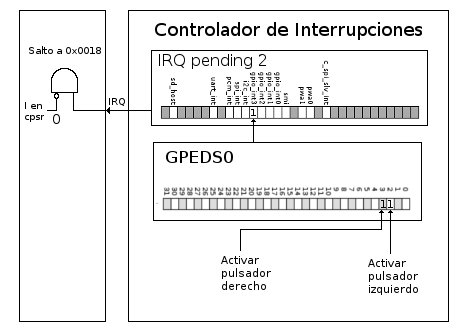
\includegraphics[width=14cm]{graphs/inter3.png}
  \caption{Interrupciones}
  \label{fig:inter3}
\end{figure}

Y el código fuente lo vemos a continuación.

\begin{lstlisting}[caption={inter3.s},label={lst:codigoPract5_3}]
        .include  "inter.inc"
.text
        ADDEXC  0x18, irq_handler
        mov     r0, #0b11010010   @modo IRQ, FIQ&IRQ desact
        msr     cpsr_c, r0
        mov     sp, #0x8000
        mov     r0, #0b11010011   @modo SVC, FIQ&IRQ desact
        msr     cpsr_c, r0
        mov     sp, #0x8000000
        ldr     r0, =GPBASE
        ldr     r1, =0b00001000000000000000000000000000
        str     r1, [r0, #GPFSEL0]
/* guia bits           xx999888777666555444333222111000*/
        ldr     r1, =0b00000000000000000000000000000001
        str     r1, [r0, #GPFSEL1]
/* guia bits           10987654321098765432109876543210*/
        mov     r1, #0b00000000000000000000011000000000
        str     r1, [r0, #GPSET0]
        mov     r1, #0b00000000000000000000000000001100
        str     r1, [r0, #GPREN0]
        ldr     r0, =INTBASE
/* guia bits           10987654321098765432109876543210*/
        mov     r1, #0b00000000000100000000000000000000
        str     r1, [r0, #INTENIRQ2]
        mov     r0, #0b01010011   @modo SVC, IRQ activo
        msr     cpsr_c, r0
bucle:  b       bucle

irq_handler:
        push    {r0, r1}
        ldr     r0, =GPBASE
/* Apaga los dos LEDs rojos  54321098765432109876543210*/
        mov     r1, #0b00000000000000000000011000000000
        str     r1, [r0, #GPCLR0]
/* Consulta si se ha pulsado el botón GPIO2 */
        ldr     r1, [r0, #GPEDS0]
        ands    r1, #0b00000000000000000000000000000100
/* Sí: Activa GPIO 9; No: Activa GPIO 10 */
        movne   r1, #0b00000000000000000000001000000000
        moveq   r1, #0b00000000000000000000010000000000
        str     r1, [r0, #GPSET0]
/* Desactivo los dos flags GPIO pendientes de atención
   guia bits                 54321098765432109876543210*/
        mov     r1, #0b00000000000000000000000000001100
        str     r1, [r0, #GPEDS0]
        pop     {r0, r1}
        subs    pc, lr, #4
\end{lstlisting}

Obviamos los dos primeros pasos (apuntar a RTI e inicialización de punteros de pila) puesto
que son idénticos al ejemplo anterior.

Lo siguiente que tenemos es configurar e inicializar los puertos del GPIO. Por un lado
ponemos los correspondientes a los LEDs rojos (GPIO 9 y GPIO 10) como salida. Por otro
lado escribimos un uno en ambos LEDs, para que al arrancar veamos los dos LEDs encendidos.
Así sabemos que el programa está cargado a la espera de que activemos los pulsadores.

\begin{lstlisting}
        ldr     r0, =GPBASE
        ldr     r1, =0b00001000000000000000000000000000
        str     r1, [r0, #GPFSEL0]
/* guia bits           xx999888777666555444333222111000*/
        ldr     r1, =0b00000000000000000000000000000001
        str     r1, [r0, #GPFSEL1]
/* guia bits           10987654321098765432109876543210*/
        mov     r1, #0b00000000000000000000011000000000
        str     r1, [r0, #GPSET0]
\end{lstlisting}

Luego habilitamos las interrupciones particulares del GPIO en el registro
{\tt GPREN0}, en concreto las que entran por los pulsadores (GPIO 2 y GPIO 3). 
Para que las peticiones se propaguen desde el GPIO al controlador de interrupciones
habilitamos el bit 20 del registro {\tt INTENIRQ2}.

\begin{lstlisting}
        mov     r1, #0b00000000000000000000000000001100
        str     r1, [r0, #GPREN0]
        ldr     r0, =INTBASE
/* guia bits           10987654321098765432109876543210*/
        mov     r1, #0b00000000000100000000000000000000
        str     r1, [r0, #INTENIRQ2]
\end{lstlisting}

Para terminar activando globalmente las IRQ y metiéndonos en el bucle infinito.

\begin{lstlisting}
        mov     r0, #0b01010011   @modo SVC, IRQ activo
        msr     cpsr_c, r0
bucle:  b       bucle
\end{lstlisting}

Veamos ahora el aspecto que tiene la RTI. Lo primero es poner los LEDs susceptibles de
encenderse (los LEDs rojos) a cero.

\begin{lstlisting}
irq_handler:
        push    {r0, r1}
        ldr     r0, =GPBASE
/* Apaga los dos LEDs rojos  54321098765432109876543210*/
        mov     r1, #0b00000000000000000000011000000000
        str     r1, [r0, #GPCLR0]
\end{lstlisting}

Testeamos cuál de los dos pulsadores se ha activado, indicándolo en el flag Z.

\begin{lstlisting}
/* Consulta si se ha pulsado el botón GPIO2 */
        ldr     r1, [r0, #GPEDS0]
        ands    r1, #0b00000000000000000000000000000100
\end{lstlisting}

En función del flag Z encendemos uno u otro LED.

\begin{lstlisting}
/* Sí: Activa GPIO 9; No: Activa GPIO 10 */
        movne   r1, #0b00000000000000000000001000000000
        moveq   r1, #0b00000000000000000000010000000000
        str     r1, [r0, #GPSET0]
\end{lstlisting}

Y finalmente desactivamos los dos flags GPIO pendientes de atención.

\begin{lstlisting}
        mov     r1, #0b00000000000000000000000000001100
        str     r1, [r0, #GPEDS0]
        pop     {r0, r1}
        subs    pc, lr, #4
\end{lstlisting}

\subsection{Parpadeo secuencial de LEDs con sonido por altavoz}

En este ejemplo vamos a trabajar con el temporizador, pero esta vez vamos a complicar
un poco las cosas. En lugar de una fuente vamos a atender simultáneamente las peticiones
de los comparadores {\tt C1} y {\tt C3}.

\begin{figure}[h]
  \centering
    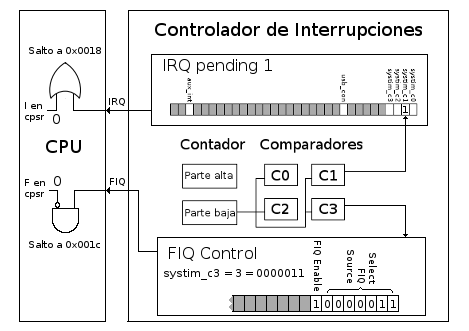
\includegraphics[width=14cm]{graphs/inter4.png}
  \caption{Interrupciones}
  \label{fig:inter4}
\end{figure}

Con esta segunda fuente vamos a controlar el altavoz, como podemos
observar en la figura \ref{fig:inter3}. Sacar un tono
puro por el altavoz es equivalente a hacer parpadear un LED, lo único que cambia es que usamos
otro pin distinto {\tt GPIO 4} y aumentamos la frecuencia para que sea audible (a 1 Hz el oído
humano no captaría sonido alguno). Utilizaremos la frecuencia estándar de afinación
de 440 Hz, que coincide con el tono de espera de marcado en telefonía fija.

Por otro lado en lugar de hacer parpadear todos los LEDs lo que haremos es repetir una
secuencia de 6 posiciones en la que en todo momento sólo uno de los 6 LEDs está encendido, que
va cambiando de izquierda a derecha (aparentando movimiento) y cuando se llegue al sexto LED
comenzamos de nuevo desde el primero. Para dar más sensación de movimiento disminuimos el periodo
a 200 milisegundos.

La clave de todo está en saber cuál de los dos comparadores ha producido la interrupción (se
puede dar el caso en que salten los dos a la vez). Ésto se puede hacer de dos formas distintas:
o bien leemos el bit asociado {\tt systim\_cx} en el registro {\tt IRQ pending 1}, o bien leemos
el {\tt Mx} del registro {\tt CS}. Elegimos el segundo caso, así no gastamos otro registro más
para almacenar {\tt INTBASE}.

El código completo del ejemplo es el siguiente.

\begin{lstlisting}[caption={inter4.s},label={lst:codigoPract5_4}]
        .include  "inter.inc"
.text
        ADDEXC  0x18, irq_handler
        mov     r0, #0b11010010   @modo IRQ, FIQ&IRQ desact
        msr     cpsr_c, r0
        mov     sp, #0x8000
        mov     r0, #0b11010011   @modo SVC, FIQ&IRQ desact
        msr     cpsr_c, r0
        mov     sp, #0x8000000
        ldr     r0, =GPBASE
        ldr     r1, =0b00001000000000000001000000000000
        str     r1, [r0, #GPFSEL0]
/* guia bits           xx999888777666555444333222111000*/
        ldr     r1, =0b00000000001000000000000000001001
        str     r1, [r0, #GPFSEL1]
        ldr     r1, =0b00000000001000000000000001000000
        str     r1, [r0, #GPFSEL2]
        ldr     r0, =STBASE
        ldr     r1, [r0, #STCLO]
        add     r1, #2
        str     r1, [r0, #STC1]
        str     r1, [r0, #STC3]
        ldr     r0, =INTBASE
        mov     r1, #0b1010
        str     r1, [r0, #INTENIRQ1]
        mov     r0, #0b01010011   @modo SVC, IRQ activo
        msr     cpsr_c, r0
bucle:  b       bucle

irq_handler:
        push    {r0, r1, r2, r3}
        ldr     r0, =STBASE
        ldr     r1, =GPBASE
        ldr     r2, [r0, #STCS]
        ands    r2, #0b0010
        beq     sonido
        ldr     r2, =cuenta
/* guia bits           10987654321098765432109876543210*/
        ldr     r3, =0b00001000010000100000111000000000
        str     r3, [r1, #GPCLR0]
        ldr     r3, [r2]          @cuenta
        subs    r3, #1
        moveq   r3, #6
        str     r3, [r2]
        ldr     r3, [r2, +r3, LSL #2]
        str     r3, [r1, #GPSET0]
        mov     r3, #0b0010
        str     r3, [r0, #STCS]
        ldr     r3, [r0, #STCLO]
        ldr     r2, =200000       @5 Hz
        add     r3, r2
        str     r3, [r0, #STC1]
        ldr     r3, [r0, #STCS]
        ands    r3, #0b0100
        beq     final
sonido: ldr     r2, =bitson
        ldr     r3, [r2]
        eors    r3, #1
        str     r3, [r2]
        mov     r3, #0b10000      @altavoz
        streq   r3, [r1, #GPSET0]
        strne   r3, [r1, #GPCLR0]
        mov     r3, #0b1000
        str     r3, [r0, #STCS]
        ldr     r3, [r0, #STCLO]
        ldr     r2, =1136         @440 Hz
        add     r3, r2
        str     r3, [r0, #STC3]
final:  pop     {r0, r1, r2, r3}
        subs    pc, lr, #4

bitson: .word   0
cuenta: .word   1
/* guia bits      7654321098765432109876543210*/
secuen: .word   0b1000000000000000000000000000
        .word   0b0000010000000000000000000000
        .word   0b0000000000100000000000000000
        .word   0b0000000000000000100000000000
        .word   0b0000000000000000010000000000
        .word   0b0000000000000000001000000000
\end{lstlisting}

Como es muy parecido al ejemplo de antes, sólo vamos a comentar las diferencias que encontremos.
La primera de ellas es que además de los 6 GPIOs de los LEDs, configuramos como salida un séptimo
pin, el GPIO 4, para manejar el altavoz.

\begin{lstlisting}
        ldr     r0, =GPBASE
        ldr     r1, =0b00001000000000000001000000000000
        str     r1, [r0, #GPFSEL0]
\end{lstlisting}

El siguiente código es para incluir el comparador {\tt C3} (además del {\tt C1} que había
anteriormente), tanto para proporcionar la primera
interrupción como para habilitarla individualmente.

\begin{lstlisting}
        ldr     r0, =STBASE
        ldr     r1, [r0, #STCLO]
        add     r1, #2
        str     r1, [r0, #STC1]
        str     r1, [r0, #STC3]
        ldr     r0, =INTBASE
        mov     r1, #0b1010
        str     r1, [r0, #INTENIRQ1]
\end{lstlisting}

Ya hemos acabado con el programa principal, veamos ahora la RTI. Primero mostramos la estructura
del código y luego las rutinas individuales tanto para el manejo de LEDs como para el
altavoz.

\begin{lstlisting}
irq_handler:
        push    {r0, r1, r2, r3}
        ldr     r0, =STBASE
        ldr     r1, =GPBASE
        ldr     r2, [r0, #STCS]
        ands    r2, #0b0010
        beq     sonido

        [ manejo de LEDs ]

        ldr     r3, [r0, #STCS]
        ands    r3, #0b0100
        beq     final
sonido:
        [ manejo de altavoz ]

final:  pop     {r0, r1, r2, r3}
        subs    pc, lr, #4
\end{lstlisting}

Los registros {\tt r0} y {\tt r1} los hacemos apuntar a la base del {\tt System Timer} y del
{\tt GPIO} y no tocamos dichos valores durante toda la interrupción, vamos a estar
constantemente leyendo y escribiendo registros y resulta incómodo tener que cargar la
base cada vez.

Es un error muy habitual suponer que la fuente de la interrupción sólo ha sido una, aunque
la gran mayoría de las veces sea así se puede dar el caso de que coincidan los dos comparadores
a la vez. De la misma forma si sabemos que sólo hay dos fuentes y una de ellas no ha
provocado la interrupción, por descarte ha tenido que ser la otra, podemos ahorrarnos la
comprobación.

El flujo sería el siguiente: leemos {\tt M1} para ver si la interrupción la ha provocado el
comparador de {\tt C1}, si ha sido así ejecutamos el código de manejo de LEDs; si no,
saltamos directamente al manejo del altavoz (sabemos seguro que la fuente viene de ahí).

Tras el código del manejo de LEDs leemos {\tt M3} para saber si además de {\tt C1} ha
saltado también el comparador {\tt C3}. Si no ha saltado, lo más normal, salimos por
{\tt final}; si lo ha hecho, procesamos la interrupción con el código de manejo del altavoz
para luego salir de la RTI.

Estos programas no son fáciles de crear y nunca funcionan a la primera. Es una buena práctica
hacer funcionar por separado el código de los LEDs y el código del altavoz, y una vez
comprobemos que funcionan, aglutinarlo en una única RTI. De esta forma aislamos lo máximo
posible los errores que podamos cometer, es muy fácil equivocarse en una tontería y estar
dándole vueltas al código sin encontrar el fallo. A diferencia de los primeros capítulos
que disponíamos de {\tt gdb}, en Bare Metal no tenemos acceso a ningún depurador.

Prosigamos ahora con el código de manejo de LEDs. Recordemos que hemos complicado un poco
las cosas para emitir una secuencia en lugar de un simple parpadeo. Para ello mostramos
el código seguido de las variables empleadas en el mismo.

\begin{lstlisting}
        ldr     r2, =cuenta
/* guia bits           10987654321098765432109876543210*/
        ldr     r3, =0b00001000010000100000111000000000
        str     r3, [r1, #GPCLR0]
        ldr     r3, [r2]          @cuenta
        subs    r3, #1
        moveq   r3, #6
        str     r3, [r2]
        ldr     r3, [r2, +r3, LSL #2]
        str     r3, [r1, #GPSET0]
        mov     r3, #0b0010
        str     r3, [r0, #STCS]
        ldr     r3, [r0, #STCLO]
        ldr     r2, =200000       @5 Hz
        add     r3, r2
        str     r3, [r0, #STC1]
        [...]
cuenta: .word   1
/* guia bits      7654321098765432109876543210*/
secuen: .word   0b1000000000000000000000000000
        .word   0b0000010000000000000000000000
        .word   0b0000000000100000000000000000
        .word   0b0000000000000000100000000000
        .word   0b0000000000000000010000000000
        .word   0b0000000000000000001000000000
\end{lstlisting}

En la variable {\tt cuenta} almacenamos un contador que va desde 6 hasta 1, que actua
como índice para el array {\tt secuen}. Al decrementar aprovechamos la propia instrucción de
resta para comprobar que se ha llegado al final de la cuenta (0), y en dicho caso
restablecemos la cuenta a 6 mediante la instrucción de ejecución condicional {\tt moveq}.

En el array secuen tenemos almacenadas las posiciones que corresponden a los LEDs dentro del
registro {\tt GPSET0}, cada posición del array es para encender un LED en concreto. Antes
de esto hemos apagado todos los LEDs enviando el valor que codifica todos los LEDs al
registro {\tt GPCLR0}.

A parte de sacar la secuencia correspondiente debemos especificar cuándo será la siguiente
interrupción. Como hicimos en el ejemplo anterior, esto se resuelve leyendo el valor del
registro {\tt STCLO}, sumándole 200000 (200 milisegundos) y escribiéndolo en el comparador
{\tt STC1}.

Acabado el código de manejo de LEDs, ya sólo falta por explicar el manejo del altavoz.

\begin{lstlisting}
sonido: ldr     r2, =bitson
        ldr     r3, [r2]
        eors    r3, #1
        str     r3, [r2]
        mov     r3, #0b10000      @altavoz
        streq   r3, [r1, #GPSET0]
        strne   r3, [r1, #GPCLR0]
        mov     r3, #0b1000
        str     r3, [r0, #STCS]
        ldr     r3, [r0, #STCLO]
        ldr     r2, =1136         @440 Hz
        add     r3, r2
        str     r3, [r0, #STC3]
        [...]
bitson: .word   0
\end{lstlisting}

Es un calco de la rutina que hacía parpadear todos los LEDs, cambiando
el valor que se envia a {\tt GPCLR0/GPSET0}, el comparador que es {\tt C3} en lugar de {\tt C1},
y el valor que sumamos al temporizador, que se corresponde a 440 Hz en vez de a 1 Hz.

\subsection{Manejo de FIQs y sonidos distintos para cada LED}

Este ejemplo es muy parecido al anterior pero con cambios sutiles. El hecho de cambiar una de
las dos IRQs por una FIQ incluso simplifica el código, ya que tienen distintas RTIs y en cada
una la fuente de interrupción es única, por lo que no hay que comprobar nada ni hacer saltos.

\begin{figure}[h]
  \centering
    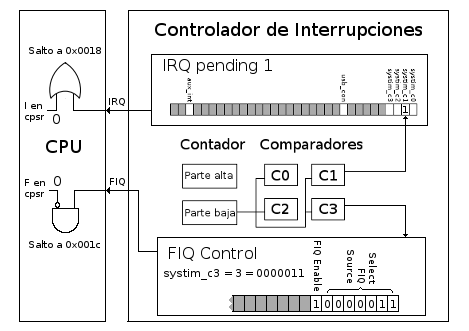
\includegraphics[width=14cm]{graphs/inter5.png}
  \caption{Interrupciones}
  \label{fig:inter5}
\end{figure}

Empecemos con el programa principal. Aquí sí que hay cambios porque tenemos que agregar un
elemento nuevo al vector de interrupciones, inicializar el puntero de pila del modo FIQ y activar
la fuente de interrupción FIQ local y globalmente.

\begin{lstlisting}[caption={Programa principal de inter5.s},label={lst:codigoPract5_5}]
        ADDEXC  0x18, irq_handler
        ADDEXC  0x1c, fiq_handler
        mov     r0, #0b11010001   @modo FIQ, FIQ&IRQ desact
        msr     cpsr_c, r0
        mov     sp, #0x4000
        mov     r0, #0b11010010   @modo IRQ, FIQ&IRQ desact
        msr     cpsr_c, r0
        mov     sp, #0x8000
        mov     r0, #0b11010011   @modo SVC, FIQ&IRQ desact
        msr     cpsr_c, r0
        mov     sp, #0x8000000
        ldr     r0, =GPBASE
        ldr     r1, =0b00001000000000000001000000000000
        str     r1, [r0, #GPFSEL0]
/* guia bits           xx999888777666555444333222111000*/
        ldr     r1, =0b00000000001000000000000000001001
        str     r1, [r0, #GPFSEL1]
        ldr     r1, =0b00000000001000000000000001000000
        str     r1, [r0, #GPFSEL2]
        ldr     r0, =STBASE
        ldr     r1, [r0, #STCLO]
        add     r1, #2
        str     r1, [r0, #STC1]
        str     r1, [r0, #STC3]
        ldr     r0, =INTBASE
        mov     r1, #0b0010
        str     r1, [r0, #INTENIRQ1]
        mov     r1, #0b10000011
        str     r1, [r0, #INTFIQCON]
        mov     r0, #0b00010011   @modo SVC, FIQ&IRQ activo
        msr     cpsr_c, r0
bucle:  b       bucle
\end{lstlisting}

Queremos que FIQ se active con {\tt C3}, que es el bit 3 del {\tt IRQ 1}, por tanto
índice 3 para la fuente {\tt FIQ}. Como veis, la única pega que tienen las FIQs es que
sólo admiten una fuente de interrupción. Además del índice ponemos el bit 7 a uno para
indicar que queremos habilitar dicha fuente, siendo la constante {\tt 0b10000011}.

Ahora veamos el manejador IRQ (la RTI) que, como hemos adelantado, es más sencilla que en el
ejemplo anterior.

\begin{lstlisting}
irq_handler:
        push    {r0, r1, r2}
        ldr     r0, =GPBASE
        ldr     r1, =cuenta
/* guia bits           10987654321098765432109876543210*/
        ldr     r2, =0b00001000010000100000111000000000
        str     r2, [r0, #GPCLR0]
        ldr     r2, [r1]          @cuenta
        subs    r2, #1
        moveq   r2, #6
        str     r2, [r1], #-4
        ldr     r2, [r1, +r2, LSL #3]
        str     r2, [r0, #GPSET0]
        ldr     r0, =STBASE
        mov     r2, #0b0010
        str     r2, [r0, #STCS]
        ldr     r2, [r0, #STCLO]
        ldr     r1, =500000       @2 Hz
        add     r2, r1
        str     r2, [r0, #STC1]
        pop     {r0, r1, r2}
        subs    pc, lr, #4
\end{lstlisting}

Observamos que al acceder a la tabla {\tt secuen} multiplicamos el índice por 8 en lugar de
por 4. Esto es así porque hemos incluído en dicha tabla el valor de la longitud de onda (inverso
de la frecuencia) con la que queremos que suene cada LED, la zona de datos es ésta.

\begin{lstlisting}
bitson: .word   0
cuenta: .word   1
secuen: .word   0b1000000000000000000000000000
        .word   716
        .word   0b0000010000000000000000000000
        .word   758
/* guia bits      7654321098765432109876543210*/
        .word   0b0000000000100000000000000000
        .word   851
        .word   0b0000000000000000100000000000
        .word   956
/* guia bits      7654321098765432109876543210*/
        .word   0b0000000000000000010000000000
        .word   1012
        .word   0b0000000000000000001000000000
        .word   1136
\end{lstlisting}

Serían las notas puras que van después del LA estándar de 440 Hz (1136), cuyos semitonos se
obtienen multiplicando la frecuencia por raíz duodécima de 2, que es aproximadamente 1,05946.
Las notas serían, en hercios: LA (440), SI (493,88), DO (523,25), RE (587,33), MI (659,26) y
FA (698,46).

Finalmente tenemos el manejador de FIQ asociado al altavoz. La elección de la fuente de
interrupción no es arbitraria, hemos escogido FIQ para el altavoz porque se ejecutará más veces
que el cambio de LEDs, concretamente 220 veces más con la nota más grave. En estos ejemplos
no importa, pero en casos reales donde el tiempo de CPU es un recurso limitado, los ciclos
que nos ahorramos con una FIQ en un proceso crítico pueden ser determinantes.

\begin{lstlisting}
fiq_handler:
        ldr     r8, =GPBASE
        ldr     r9, =bitson
        ldr     r10, [r9]
        eors    r10, #1
        str     r10, [r9], #4
        ldr     r10, [r9]
        ldr     r9, [r9, +r10, LSL #3]
        mov     r10, #0b10000     @altavoz
        streq   r10, [r8, #GPSET0]
        strne   r10, [r8, #GPCLR0]
        ldr     r8, =STBASE
        mov     r10, #0b1000
        str     r10, [r8, #STCS]
        ldr     r10, [r8, #STCLO]
        add     r10, r9
        str     r10, [r8, #STC3]
        subs    pc, lr, #4
\end{lstlisting}

El código sería idéntico al de una IRQ si no fuera porque empleamos registros a partir de
{\tt r8} en lugar de a partir de {\tt r0}, y no los salvaguardamos con las instrucciones
{\tt push/pop}. La razón es que el modo de operación FIQ es el único que tiene sus propios
registros {\tt r8-r12} (ver figura \ref{fig:tablareg}) con el objetivo de no perder el tiempo
guardando y recuperando datos de la pila. En situaciones más críticas podemos incluso ubicar
la RTI justo al final del vector de interrupciones. Esta tabla no contiene datos, sino instrucciones,
y lo que hace la CPU cuando ocurre una excepción es saltar (ejecutar) a la dirección asociada en
dicho vector. Así que cada elemento es una instrucción de salto que apunta a su RTI
correspondiente, de no ser un salto se solaparía con el siguiente elemento del vector. Excepto
el último elemento del vector, que no se solaparía con nada y que corresponde a las
interrupciones FIQ. Se ha escogido intencionalmente así para ahorrarse el salto inicial.

\subsection{Control de luces/sonido con pulsadores en lugar temporizadores}

Los pulsadores izquierdo y derecho de nuestra placa externa están asociados a los
puertos {\tt GPIO 2} y {\tt GPIO 3} respectivamente. Veremos
cómo se genera una interrupción al pulsar cualquiera de los mismos.

\begin{figure}[h]
  \centering
    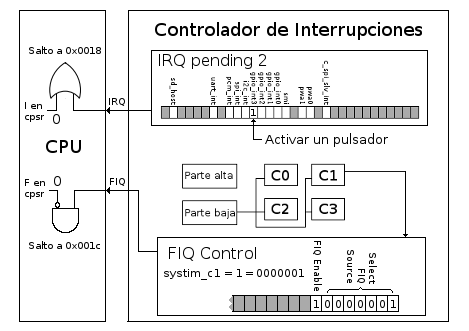
\includegraphics[width=14cm]{graphs/inter6.png}
  \caption{Interrupciones}
  \label{fig:inter6}
\end{figure}

El programa principal sería el siguiente.

\begin{lstlisting}[caption={Programa principal de inter6.s},label={lst:codigoPract5_6}]
        .include  "inter.inc"
.text
        ADDEXC  0x18, irq_handler
        ADDEXC  0x1c, fiq_handler
        mov     r0, #0b11010001   @modo FIQ, FIQ&IRQ desact
        msr     cpsr_c, r0
        mov     sp, #0x4000
        mov     r0, #0b11010010   @modo IRQ, FIQ&IRQ desact
        msr     cpsr_c, r0
        mov     sp, #0x8000
        mov     r0, #0b11010011   @modo SVC, FIQ&IRQ desact
        msr     cpsr_c, r0
        mov     sp, #0x8000000
        ldr     r0, =GPBASE
        ldr     r1, =0b00001000000000000001000000000000
        str     r1, [r0, #GPFSEL0]
/* guia bits           xx999888777666555444333222111000*/
        ldr     r1, =0b00000000001000000000000000001001
        str     r1, [r0, #GPFSEL1]
        ldr     r1, =0b00000000001000000000000001000000
        str     r1, [r0, #GPFSEL2]
/* guia bits           10987654321098765432109876543210*/
        mov     r1, #0b00000000000000000000001000000000
        str     r1, [r0, #GPSET0]
        mov     r1, #0b00000000000000000000000000001100
        str     r1, [r0, #GPREN0]
        ldr     r0, =STBASE
        ldr     r1, [r0, #STCLO]
        add     r1, #2
        str     r1, [r0, #STC1]
        ldr     r0, =INTBASE
/* guia bits           10987654321098765432109876543210*/
        mov     r1, #0b00000000000100000000000000000000
        str     r1, [r0, #INTENIRQ2]
        mov     r1, #0b10000001
        str     r1, [r0, #INTFIQCON]
        mov     r0, #0b00010011   @modo SVC, FIQ&IRQ activo
        msr     cpsr_c, r0
bucle:  b       bucle
\end{lstlisting}

Lo nuevo que vemos aquí es una escritura en el registro {\tt GPREN0}. De esta forma
le decimos al controlador de interrupciones que esos pines del GPIO serán los únicos que
provoquen interrupciones, concretamente flancos con de subida síncronos (justo
en el momento en que el botón toca fondo).

El manejador FIQ es idéntico al del ejemplo anterior, saca el sonido que corresponde al LED
por el altavoz, cambiando {\tt C3} por {\tt C1}.

Lo más relevante de este ejemplo está en la RTI asociada a la IRQ, que es la siguiente.

\begin{lstlisting}
irq_handler:
        push    {r0, r1, r2}
        ldr     r0, =GPBASE
        ldr     r1, =cuenta
        ldr     r2, =0b00001000010000100000111000000000
        str     r2, [r0, #GPCLR0]
        ldr     r2, [r0, #GPEDS0]
        ands    r2, #0b00000000000000000000000000001000
        beq     incre
        str     r2, [r0, #GPEDS0]
        ldr     r2, [r1]          @cuenta
        subs    r2, #1
        moveq   r2, #6
        b       conti
incre:  mov     r2, #0b00000000000000000000000000000100
        str     r2, [r0, #GPEDS0]
        ldr     r2, [r1]          @cuenta
        add     r2, #1
        cmp     r2, #7
        moveq   r2, #1
conti:  str     r2, [r1], #-4
        ldr     r2, [r1, +r2, LSL #3]
        str     r2, [r0, #GPSET0]
        pop     {r0, r1, r2}
        subs    pc, lr, #4
\end{lstlisting}

Tenemos una bifurcación (saltos condicionales) debido a que cada botón es una fuente distinta
de interrupción y tenemos que distinguir qué botón se ha pulsado. Aquí por suerte tenemos
un registro totalmente análogo al {\tt STCS} de los temporizadores. Se llama {\tt GPEDS0}
(también hay otro {\tt GPEDS1} para los GPIOs de 32 a 53 que no necesitamos) y sirve tanto
para saber qué fuente ha producido la interrupción como para resetear su estado (y así permitir
volver a ser interrumpidos por el mismo pin GPIO).

Con la instrucción {\tt ands} comprobamos si un determinado bit está a 1 y lo indicamos en el
flag Z. También podría valer la instrucción {\tt tst}, que tiene la ventaja de no destruir
el registro a la salida (de la misma forma que {\tt cmp} es el equivalente no destructivo de
{\tt subs}).

Y por último debemos sacar la secuencia inversa a la que teníamos para que al pulsar el
botón izquierdo las luces vayan hacia la izquierda y que con el botón derecho vayan en el otro
sentido. Si la secuencia de izquierda a derecha era  (6, 5, 4, 3, 2, 1, 6, 5, 4...), la
inversa sería (1, 2, 3, 4, 5, 6, 1...). Es decir, incrementamos y cuando llegamos a 7
lo convertimos en 1. Ésto se hace con el siguiente fragmento.

\begin{lstlisting}
        add     r2, #1
        cmp     r2, #7
        moveq   r2, #1
\end{lstlisting}

Nótese que aquí la opción destructiva {\tt subs} (en lugar de {\tt cmp}) no nos vale porque
necesitamos el valor del registro después. Sí que podemos cambiarlo por un {\tt teq} (la
alternativa no destructiva de {\tt eors}).

\section{Ejercicios}

\subsection{Todo con IRQs}

Modifica el último ejemplo ({\tt inter5.s}) para controlar el altavoz también con IRQs,
prescindiendo totalmente de las interrupciones FIQs.

\subsection{Alargar secuencia a 10 y parpadeo}

Partiendo de {\tt inter5.s} (o del resultado del ejercicio anterior) haz las siguientes
modificaciones. Si te resulta más cómodo, realízalas por orden.

\begin{itemize}
  \item Sacar de la secuencia el LED 6 (el de más a la derecha) y ponerlo a parpadear
        continuamente con una cadencia de un segundo. En este momento tendrás que acortar
        la secuencia a 5.
  \item Duplica la secuencia a 10. Para ello utiliza el código Morse aplicado a los dígitos
        (todos tienen longitud 5). Cambia el punto (tono corto) por LED apagado y el guión
        (tono largo) por LED encendido. Por supuesto los nuevos códigos tendrán su sonido
        asociado, sigue las notas (saltándote sostenidos y bemoles) para completar la tabla.
\end{itemize}

\subsection{Tope de secuencia y limitar sonido}

Partiendo de {\tt inter5.s} (o del resultado del ejercicio anterior) haz las siguientes
modificaciones. Si te resulta más cómodo, realízalas por orden.

\begin{itemize}
  \item Hasta ahora si llegamos al límite de la secuencia hemos comenzado por el principio,
        haciendo que la secuencia sea circular tanto en un sentido como en otro. Pues bien,
        ahora tienes que detectar dichos límites (tanto superior como inferior), poniendo
        una especie de tope al llegar al límite, que impida avanzar más. En caso de intentar
        avanzar en el sentido prohibido al llegar a un tope, en lugar de sacar el sonido que
        corresponda por el altavoz, auméntalo una escala (tope superior) o disminúyelo también
        una escala (tope inferior).
  \item Como habrás observado el sonido continuo resulta un tanto molesto después de un tiempo.
        Y con la indicación de los LEDs tenemos información suficiente para saber en qué
        posición de la secuencia estamos. Altera el programa para que sólamente suene el altavoz
        mientras el botón está pulsado, o lo que es lo mismo, para el sonido del altavoz cuando
        detectes un flanco de bajada en la señal GPIO correspondiente.
\end{itemize}

\subsection{Reproductor de melodía sencilla}

Escoge una melodía sencilla y trata de interpretarla. Emplea los LEDs a tu gusto para que
cambien según la nota que esté sonando. Implementa las siguientes funciones en los pulsadores.

\begin{itemize}
  \item \textbf{Pulsador izquierdo.} Cambio de tempo. La melodía debe comenzar a tempo normal (llamémoslo 1),
        y variar desde tempo lento (0) y tempo rápido (2) según la secuencia (0, 1, 2, 0...) cada
        vez que pulsemos dicho botón.
  \item \textbf{Pulsador derecho.} Iniciar/Parar/Reanudar. La melodía tiene una duración determinada y
        cuando acaba deja de sonar, no suena en modo bucle todo el tiempo. Si pulsamos dicho botón
        cuando está en silencio después que haya sonado la melodía, la función correspondiente
        sería la de iniciarla. Si lo pulsamos durante la reproducción actuaría a modo de pause
        (los LEDs se quedan congelados en el estado en el que estén), parando y reanudando la
        reproducción de la música.
\end{itemize}

En este ejemplo puedes profundizar todo lo que quieras. Por ejemplo empieza codificando los
silencios, éstos son muy importantes y también forman parte de la melodía. Un segundo paso sería
codificar la duración de las notas, si no lo has hecho ya. También es posible tener varios
instrumentos sonando a la vez, aunque sólo dispongamos de un altavoz, busca por internet {\tt
1-bit music} o {\tt beeper music} si quieres saber cómo se hace.

\chapterend{}
